\documentclass[aspectratio=43]{beamer}
\usepackage[english]{babel}
\input{chapters/preamble}
\title{Solid State Physics} %->->->->-> Check hyperref title <-<-<-<-<-
\subtitle{Presentation}
\author[Vaishnav Sankar K]{Vaishnav Sankar K}
\institute[RIEM]{
    Regional Institute of Education Mysore\\DP190014
} %You can change the Institution if you are from somewhere else
\date{\today}
%\logo{
\includegraphics[width= 0.05\textwidth]{images/a-logo.png}}

\begin{document}
    
    \frame{\titlepage}
    
    \begin{frame}{Summary}
        \begin{itemize}
        \item Elastic wave in [111] direction
        \item Experimental determination of elastic constants
        \end{itemize}
    \end{frame}
    
%%%%%%%%%%%%%%%%%%%%%%%%%%%%%%%%%%%%%%%%%%%%%%%%%%%%%%%

% Slide 1: Introduction to [111] direction
\section{Elastic wave in [111] direction}
\begin{frame}{The [111] Direction}
    \begin{itemize}
        \item Miller indices like [100], [110], and [111] describe crystal orientations.
        \item The [111] direction in a cubic crystal (FCC or BCC) is along a body diagonal.
        \item For an FCC crystal, the [111] direction cuts through atoms equally along the x, y, and z axes.
    \end{itemize}
    \begin{figure}
        \centering
        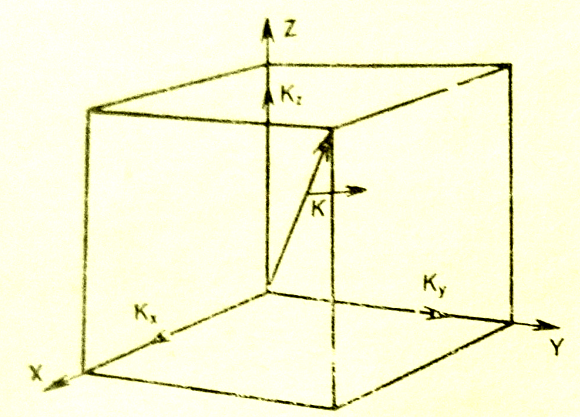
\includegraphics[width=0.5\linewidth]{images/2.png}
        \caption{Wave vector $\vec{k}$ along [111] direction}
    \end{figure}
\end{frame}

% Slide 2: Waves in the [111] direction
\begin{frame}{Waves in the [111] Direction}
    \begin{itemize}
        \item Phonon propagation in the [111] crystallographic direction.
        \item Waves can be longitudinal (compression) or transverse (shear).
        \item There are two degenerate transverse modes and a longitudinal mode.
    \end{itemize}
    \begin{figure}
        \centering
        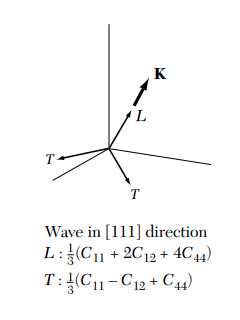
\includegraphics[width=0.3\linewidth]{images/1.png}
    \end{figure}
\end{frame}

% Slide 3: Longitudinal waves in [111] direction
\begin{frame}{Types of Waves in [111] Direction}
    \textbf{For longitudinal waves:}
    \begin{itemize}
        \item Particle motion and wave velocity are both along the [111] direction.
        \item Displacement components: $U = V = W$.
    \end{itemize}
    \vspace{0.3cm}
      \textbf{For transverse waves:}
    \begin{itemize}
        \item Particle motion and wave velocity are perpendicular to each other.
        \item Displacement components: $U = -V$ and $W=0$.
    \end{itemize}
\end{frame}

% Slide 4: Solution to longitudinal wave equation
\begin{frame}{Equations of an elastic wave}
    \textbf{Equation of motion:}
    \begin{equation}\notag
        \rho \frac{\partial^2 U}{\partial t^2} = C_{11} \frac{\partial^2 U}{\partial x^2} + C_{44} \left(\frac{\partial^2 U}{\partial y^2} + \frac{\partial^2 U}{\partial z^2}\right) + (C_{12} + C_{44})\left(\frac{\partial^2 V}{\partial x \partial y} + \frac{\partial^2 W}{\partial x \partial z}\right)
    \end{equation}
    Displacement equations:
    \begin{equation}
        U = U_0 e^{i(k_x x + k_y y + k_z z - \omega t)}
    \end{equation}
    \begin{equation}
        V = V_0 e^{i(k_x x + k_y y + k_z z - \omega t)}
    \end{equation}
        \begin{equation}
        W = W_0 e^{i(k_x x + k_y y + k_z z - \omega t)}
    \end{equation}
\end{frame}

 
\begin{frame}{Wave vector} 
In a cubic crystal, wave vector components are related: $k_x = k_y =k_z$

Therefore,
\begin{align*}
k_x^2 + k_y^2 + k_z^2 &= 3 k_x^2 = k^2\\
k_x^2 & = \frac{k^2}{3}\\
k_x & = \frac{k}{\sqrt{3}}
\end{align*}

Now, the displacement equations are: 
\begin{equation}
    \tag{3}
    U =  U_0 e^{i\left(\frac{k}{\sqrt{3}}(x+y+z) - \omega t\right)}
    \label{eq3}
\end{equation}

\begin{equation}
    \tag{4}
    V =  V_0 e^{i\left(\frac{k}{\sqrt{3}}(x+y+z) - \omega t\right)}
    \label{eq4}
\end{equation}

\begin{equation}
    \tag{5}
    W =  W_0 e^{i\left(\frac{k}{\sqrt{3}}(x+y+z) - \omega t\right)}
    \label{eq5}
\end{equation}
\end{frame}


\begin{frame}
    \begin{figure}
        \centering
        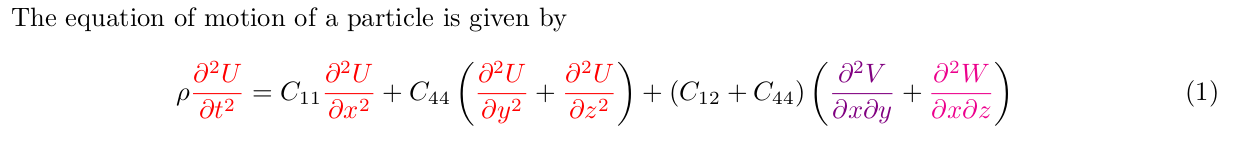
\includegraphics[width=\linewidth]{images/5.png}
    \end{figure}
\end{frame}

\begin{frame}
       \begin{figure}
        \centering
        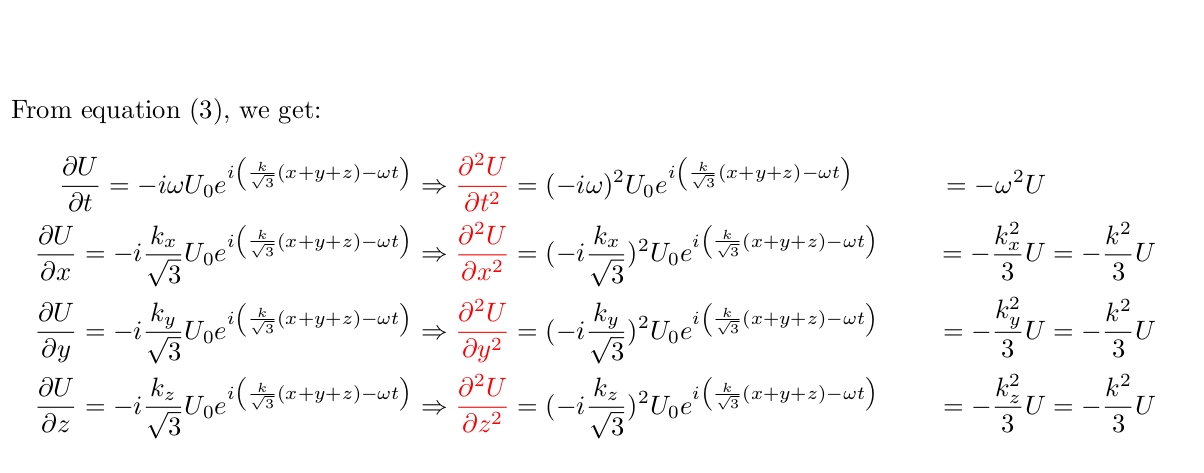
\includegraphics[width=\linewidth]{images/6.png}
    \end{figure}
\end{frame}

\begin{frame}
       \begin{figure}
        \centering
        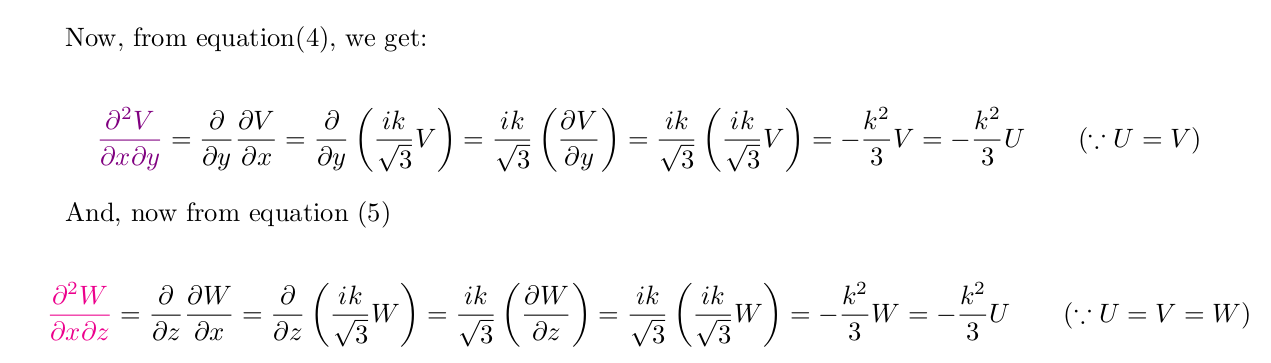
\includegraphics[width=\linewidth]{images/7.png}
    \end{figure}
\end{frame}
 
 
 \begin{frame}
       \begin{figure}
        \centering
        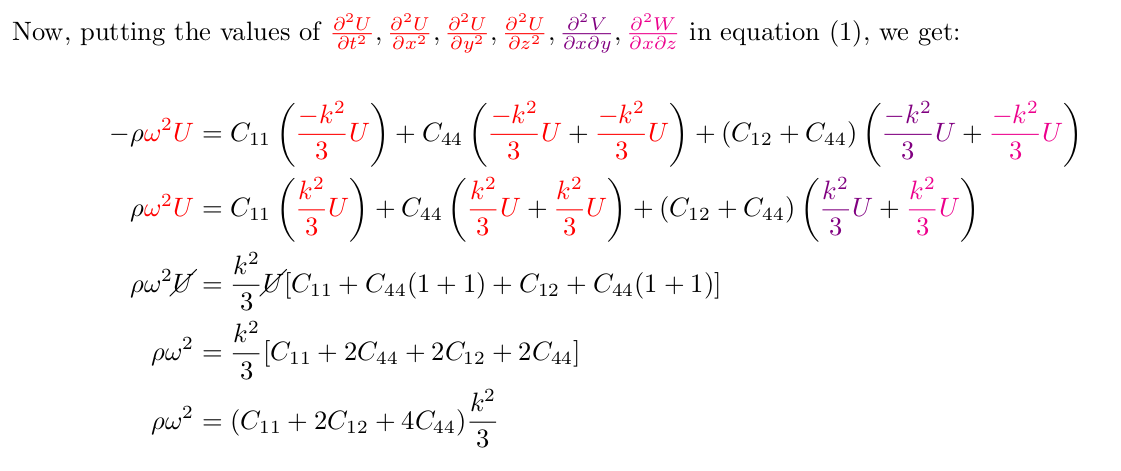
\includegraphics[width=\linewidth]{images/8.png}
    \end{figure}
\end{frame}

 \begin{frame}
       \begin{figure}
        \centering
        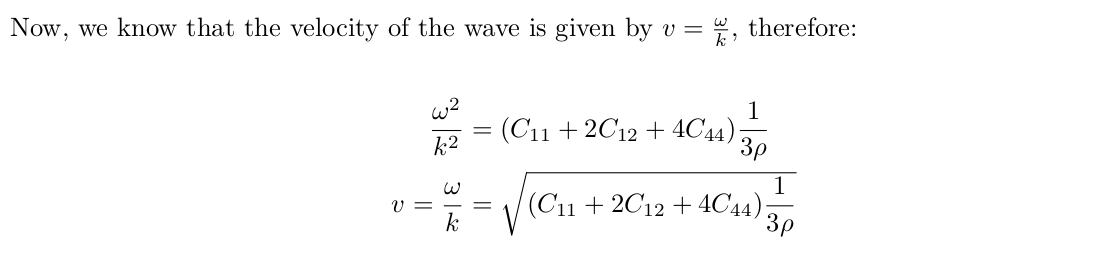
\includegraphics[width=\linewidth]{images/9.png}
    \end{figure}
    \textbf{This is the velocity of a longitudinal elastic wave in [111] direction of a cubic crystal}
\end{frame}





 \begin{frame}{Transverse wave in [111] direction}
       \begin{figure}
        \centering
        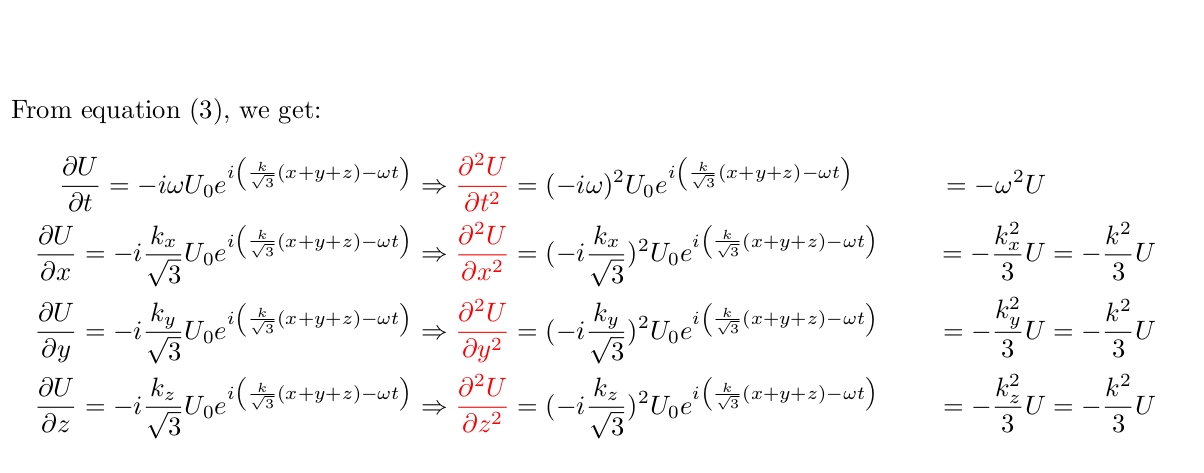
\includegraphics[width=\linewidth]{images/6.png}
    \end{figure}
\end{frame}


 \begin{frame}
 \textbf{From equation(4) we get:}
       \begin{figure}
        \centering
        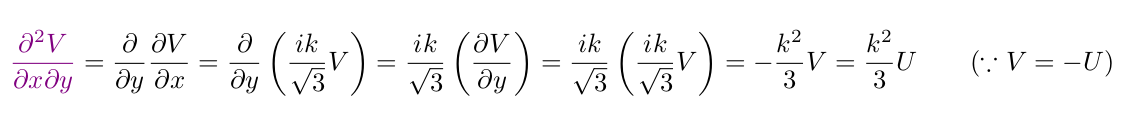
\includegraphics[width=\linewidth]{images/10.png}
    \end{figure}
    \textbf{From equation(5) we get:}
    \begin{figure}
        \centering
        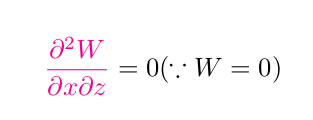
\includegraphics[width=0.3\linewidth]{images/11.png}
    \end{figure}
\end{frame}

 \begin{frame}
       \begin{figure}
        \centering
        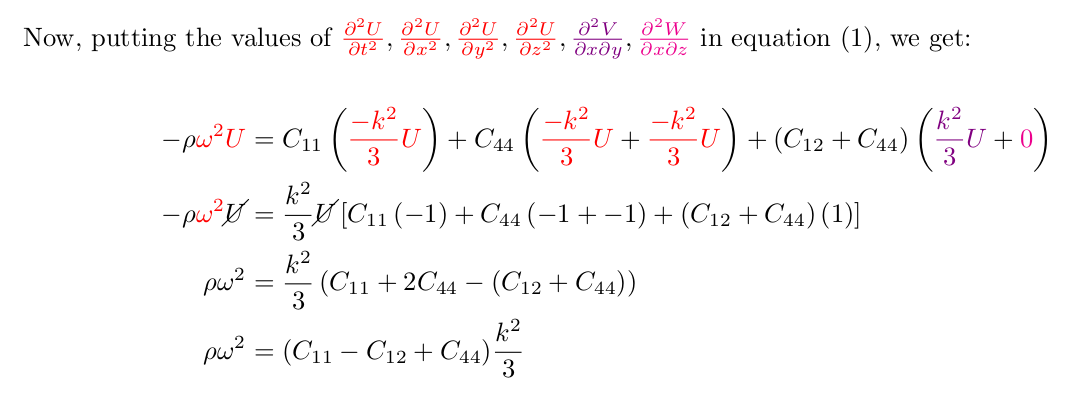
\includegraphics[width=\linewidth]{images/12.png}
    \end{figure}
\end{frame}

 \begin{frame}
       \begin{figure}
        \centering
        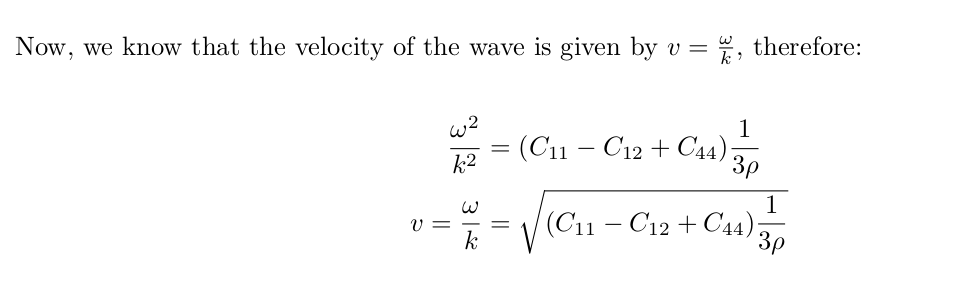
\includegraphics[width=\linewidth]{images/13.png}
    \end{figure}
    \textbf{This is the velocity of transverse wave in [111] direction}
\end{frame}

\section{Experimental Determination of Elastic Constants}

\begin{frame}{Relation Between Velocities and Elastic Constants}
    \begin{itemize}
        \item Elastic waves' velocities and elastic moduli help in determining elastic constants.
        \item Elastic waves are excited in a crystal, and their velocity is measured.
    \end{itemize}
\end{frame}

\begin{frame}{Ultrasonic Pulse Method}
    \begin{itemize}
        \item Frequencies are in the ultrasonic range, where the crystal behaves as a continuous elastic medium.
        \item The waves are pulsed; this is known as the ultrasonic pulse method.
    \end{itemize}
    \begin{figure}[H]
        \centering
        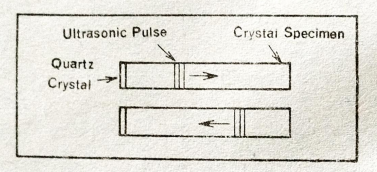
\includegraphics[scale=0.5]{images/3.png}
    \end{figure}
\end{frame}

\begin{frame}{Crystal Specimen Setup}
    \begin{itemize}
        \item The crystal specimen has flat ends for proper pulse reflection.
        \item A piezoelectric quartz transducer is attached to one end.
    \end{itemize}
\end{frame}

\begin{frame}{Pulse Reflection and Velocity Measurement}
    \begin{itemize}
        \item The ultrasonic pulse is reflected from the rear surface back to the transducer.
        \item Time taken for the pulse to travel round-trip is measured electronically.
        \item Velocity is calculated using distance divided by time.
    \end{itemize}
\end{frame}

\begin{frame}{Apparatus of ultrasonic pulse-echo method}
    \begin{figure}[H]
        \centering
        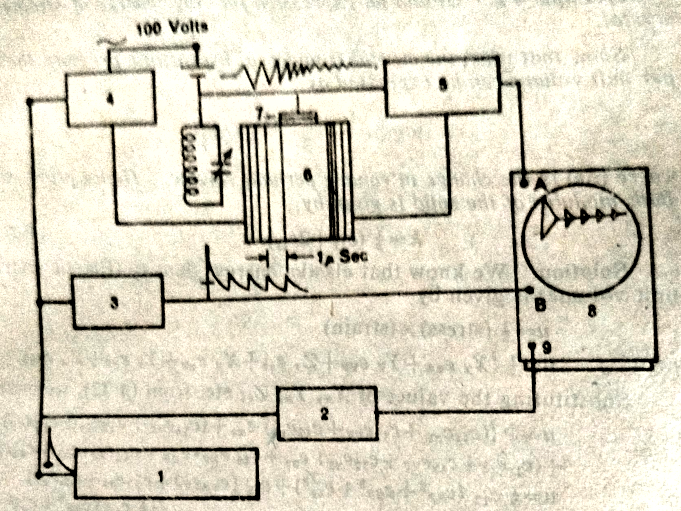
\includegraphics[scale=0.23]{images/4.png}
        \caption{Block diagram of apparatus for ultrasonic pulse-echo method.  1.trigger generator(1000$\mu$ s period, 2. delay circuit, 3. time mark generator, 4. thyratron switch, 5. wide band rf amplifier, 6.specimen, 7.quartz, 8.oscilloscope, 9.sweep trigger}
    \end{figure}
\end{frame}

\begin{frame}{Electronic Apparatus and Measurement Process}
    \begin{itemize}
        \item The trigger generator initiates the process by discharging a condenser through an LC network.
        \item A voltage wave is imposed on the quartz transducer glued to the specimen.
    \end{itemize}
\end{frame}

\begin{frame}{Measurement Accuracy}
    \begin{itemize}
        \item The time mark generator and delay circuit ensure precise measurement of pulse arrival.
        \item This method is highly accurate and uses only small specimen sizes.
    \end{itemize}
\end{frame}

\begin{frame}{Applications and Elastic Constants}
    \begin{itemize}
        \item This method can determine elastic constants at various temperatures and pressures.
        \item Elastic stiffness constants $C_{11}, C_{12}, C_{44}$ of a cubic crystal can be calculated.
    \end{itemize}
\end{frame}

    
%%%%%%%%%%%%%%%%%%%%%%%%%%%%%%%%%%%%%%%%%%%%%%%%%%%%    
    
    
    \section*{References} %You can remove this if you do not want to use it
       % \nocite{Djairo} \nocite{PhilPanof} \nocite{Fleming} \nocite{Shankar}
        \begin{frame}{References}
            \begin{itemize}
            \item Hemarajini and Kakani, Solid State Physics
            \item Charles Kittel, Solid State Physics
            \item Circus of Physics Channel
            \end{itemize}
        \end{frame}

    \section{}
    \begin{frame}{}
        \centering
            \Huge\bfseries
        \textcolor{orange}{The End}
    \end{frame}
\end{document}
